\documentclass[../main.tex]{subfiles}

\begin{document}

\chapter{Model Data} \label{model_data}

In this section, we describe the data sources used in our project, and identify specific features to be used in our sector classification heuristic. Additionally, we also describe the benchmark sector classification universe that we will use to evaluate our final results. This section begins the discussion of our first research goal, RG-1.
  
 \begin{table}[h!]
    \centering
    \begin{tabular}{| c | c |}
        \hline
        &  \\
        RG-1 & Utilize data-driven algorithms to derive a truly objective classification heuristic. \\
        & \\
        \hline
    \end{tabular}
\end{table}

\section{Fundamentals Data Overview}

In the previous section (see page~\pageref{literature_review:economic_sectors_fundamentals}), we explored the effect of the violation of the Modigliani-Miller theoretic universe conditions on the capital structure irrelevance principle, in conjunction with observations of the dynamics of the determinants of capital structure in transitional and established economies. The logical corollary of this analysis is that fundamentals data reflective of capital structure - particularly those specific to the Modigliani-Miller universe conditions - are optimal descriptors of the economic domain of a company.

Based on this conclusion, we idenfied earnings data from Form 10-K\citeFormat{\cite{U.S.SecuritiesandExchangeCommission2019Form10-K}} filings to be our model input data. This data was retrieved for 362 companies in the S\&P 500 Index, for every year from 2010 to 2017, from the Compustat Database\citeFormat{\cite{SPGlobalMarketIntelligence2019CompustatIntelligence}}, via the Wharton Research Data Services\citeFormat{\cite{TheWhartonSchool1993WhartonServices}} Cloud (hereafter \textit{WRDS}).

\section{Feature Selection}

Given the variability of earnings reports, we identified 15 specific features from the annual Balance Sheet, Income Statement, and Statement of Cash Flows guaranteed to exist for all companies in our dataset. In addition to being common across all companies, they were also isolated on the basis of being related to, or direct arguments of, the capital structure of the company.

\begin{table}[h]
    \centering
    \begin{tabular}{|c|c|c|}
        \hline
        Total Assets & Cash \& Equivalents & Receivables \\
        \hline
        Inventories & Sales & Cost of Goods Sold \\
        \hline
        Gross Profit & Operating Cash Flow & Operating Income \\
        \hline
        Depreciation, Depletion \& Amortization & Interest Expense & Non-Operating Income/Expense \\
        \hline
        Income Taxes & Advertising Expense & Research \& Development Expense \\
        \hline
    \end{tabular}
    \caption{Selected model input data features from Form 10-K for each company.}
    \label{table:model_data:features}
\end{table}

\pagebreak

\begin{figure}[h]
    \centering
    \fbox{
    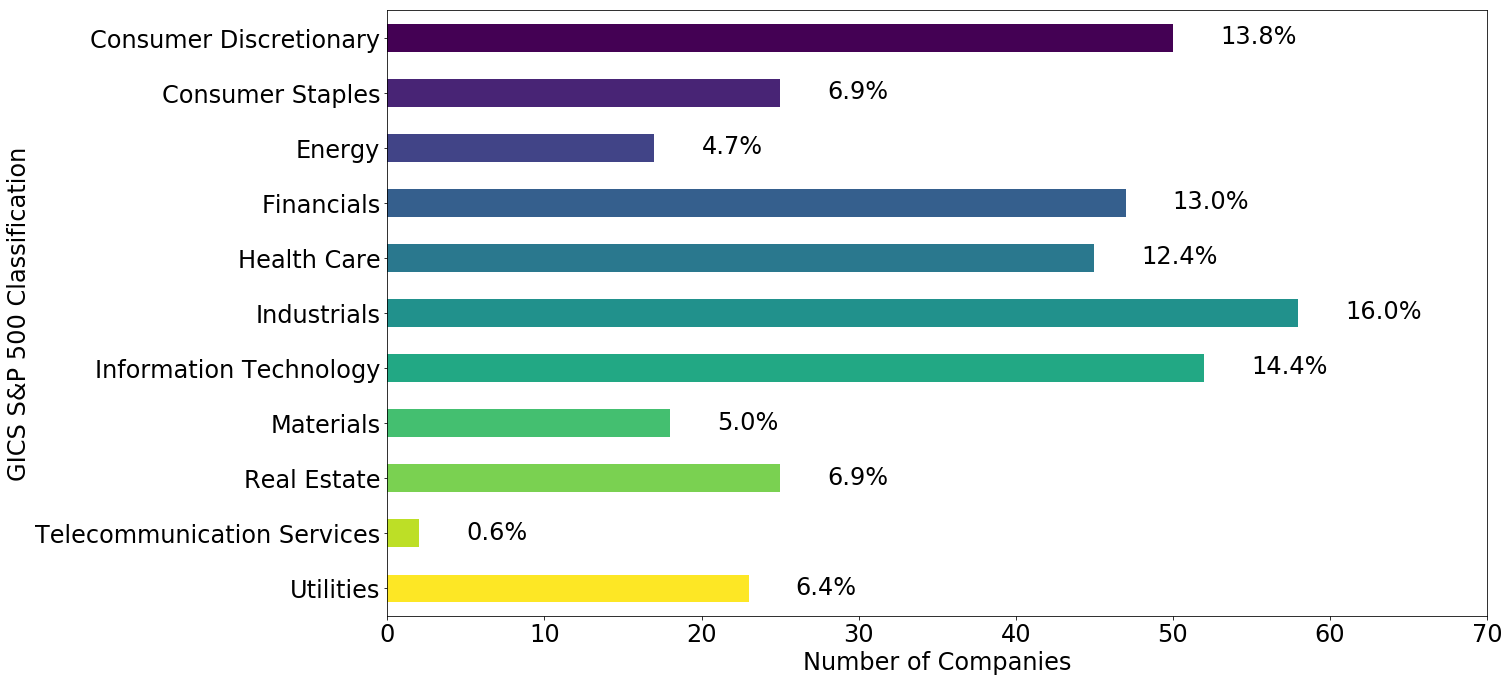
\includegraphics[width=.9\linewidth]{images/sp500_sector_distribution.png}
    }
    \caption{Distribution of input data companies ($n = 362$) across sectors in the benchmark universe (i.e. GICS S\&P 500 Classification).}
    \label{fig:model_data:sp500_sector_distribution}
\end{figure}

\section{Benchmark Sector Universe}

To evaluate our final learned sector universe and fully address RG-3, we identified the GICS S\&P 500 Classification\citeFormat{\cite{MSCI-MorganStanleyCapitalInternational2019GICSMSCI}} (hereafter \textit{benchmark universe}) to be our benchmark. Unfortunately, the complete dataset of sector assignments our benchmark universe is proprietary. Due to this, we were unable to collate historical sector assignments, and were limited to the latest sector assignments for companies in our input data space.

Due to the disparity in temporal alignment between our data, we decided to utilize only the latest available data for our learned sector universe evlautions. That is - unless stated otherwise - we only utilized learned sector assignments implied by the 2017 10-K Form data for the remainder of this project.

The distribution of the 362 companies in our input data across various sectors in the benchmark universe is displayed in Figure~\ref{fig:model_data:sp500_sector_distribution}.

\end{document}